% This is samplepaper.tex, a sample chapter demonstrating the
% LLNCS macro package for Springer Computer Science proceedings;
% Version 2.20 of 2017/10/04
%
\documentclass[runningheads]{llncs}
%
\usepackage{graphicx}
% Used for displaying a sample figure. If possible, figure files should
% be included in EPS format.
%
% If you use the hyperref package, please uncomment the following line
% to display URLs in blue roman font according to Springer's eBook style:
% \renewcommand\UrlFont{\color{blue}\rmfamily}

\begin{document}
% %
% \title{Contribution Title\thanks{Supported by organization x.}}
% %
% %\titlerunning{Abbreviated paper title}
% % If the paper title is too long for the running head, you can set
% % an abbreviated paper title here
% %
% \author{First Author\inst{1}\orcidID{0000-1111-2222-3333} \and
% Second Author\inst{2,3}\orcidID{1111-2222-3333-4444} \and
% Third Author\inst{3}\orcidID{2222--3333-4444-5555}}
% %
% \authorrunning{F. Author et al.}
% % First names are abbreviated in the running head.
% % If there are more than two authors, 'et al.' is used.
% %
% \institute{Princeton University, Princeton NJ 08544, USA \and
% Springer Heidelberg, Tiergartenstr. 17, 69121 Heidelberg, Germany
% \email{lncs@springer.com}\\
% \url{http://www.springer.com/gp/computer-science/lncs} \and
% ABC Institute, Rupert-Karls-University Heidelberg, Heidelberg, Germany\\
% \email{\{abc,lncs\}@uni-heidelberg.de}}
% %
% \maketitle              % typeset the header of the contribution
% %
\begin{abstract}
....
% The abstract should briefly summarize the contents of the paper in
% 150--250 words.

% \keywords{First keyword  \and Second keyword \and Another keyword.}
\end{abstract}
% %
% %
% %
\section{Introduction}
Watersheds, with their common points of drainage and collection into downstream environments, are important to the modeling of environmental change and runoff of pollutants.
Software models have long been used to estimate changes to watersheds.
These models typically involve defining physical characteristics of the watershed such as elevation, drainage patterns, and soil types, along with a calibration step against measured environmental data.

In this paper, we examine methods to encapsulate and package existing modeling approaches using a multivariate random forest regression approach.
The aim is to predict yearly changes in runoff can be predicted from changes in precipitation or forestry.
The end result captures the mathematical modeling of a traditional hydrology transport model, while allowing us to isolate specific predictors and their impact on a variety of measured downstream pollutants.
Furthermore, we present a standard way of packaging these models so that end-users, such as policy makers, can make land-use decisions without the requisite technical knowledge to calibrate hydrology models.

\section{Materials and Methods}
\subsection{Study Area}
The South Nation Watershed spans 381,100 hectares between the Ottawa River to the watershed's North and the St. Lawrence River to the South.
Mostly comprised of farm fields, the watershed drains both into the South Nation River, with eventual confluence at the Ottawa River, and into the Little Castor River.
The watershed has been of increasing importance in recent years because of the wide-spread agricultural use and urbanization in towns along the South Nation River from such as Chesterville, Casselman, and Plantaganet along the South Nation River.

\subsection{Hydrological Modeling}
% SWAT Models + How they were built
In order to encompass topographic and other physical characteristics of the watershed, we built a general purpose rainfall model using the Soil and Water Assessment Tool (SWAT) and used outputs from the SWAT model to train random forest models.
The resulting steps were:

\begin{enumerate}
	\item Setup of a rainfall model using the Soil and Water Assessment Tool (SWAT)
	\item Calibration of the SWAT model using measured water quality data
	\item Simulation of runoffs using the SWAT model
	\item Fitting random forest models using the simulated values from SWAT
	\item Evaluating the models' accuracies using a Time Series Split
	\item Generating final random forest models and packaging into a application for end-users
\end{enumerate}

After creating the SWAT model, it was calibrated using water quality data from the Ontario Provincial (Stream) Water Quality Monitoring Network, and outputs were simulated from the model.
The final predictands from our SWAT model were: water outflow rate, evaporation rate, water transmission loss rate, sediment output, sediment concentration, organic nitrogen output, organic phosphorus output, nitrate output, ammonium output, nitrogen dioxide output, mineral phosphorus output, chlorophyll alpha output, carbonaceous biochemical oxygen demand of material output, dissolved oxygen output, and total nitrogen in surface runoff.

% random forest models
Using the simulated values from SWAT, we fitted a random forest model for each predictand.
For predictors, we isolated the forest cover and precipitation for each subbasin in the watershed; with 31 subbasins, this creates 62 individual predictors for the random forest model, though not all predictors are included as nodes in the model after training.
The random forest models were created using Scikit-Learn (SKLearn), a Python-based machine learning library.
% Packaging
Flask, a server-side web framework, ReactJS, a client-side JavaScript library, and Docker, a virtualization program, was used to package the models for access through a web browser by end-users.

\section{Results}
\subsection{Interface}
The models are accessible to users via any standard web browser.
Users can enter measured or expected precipitation metrics across the watershed, and individual forest cover metrics per subbasin.
The software can then predict, within seconds, the expected downstream runoff measures for the aforementioned predictands and present the results to users as shown in Figure \ref{fig-web}.

\begin{figure}[h]
\begin{center}
\minipage{1.0\textwidth}%
  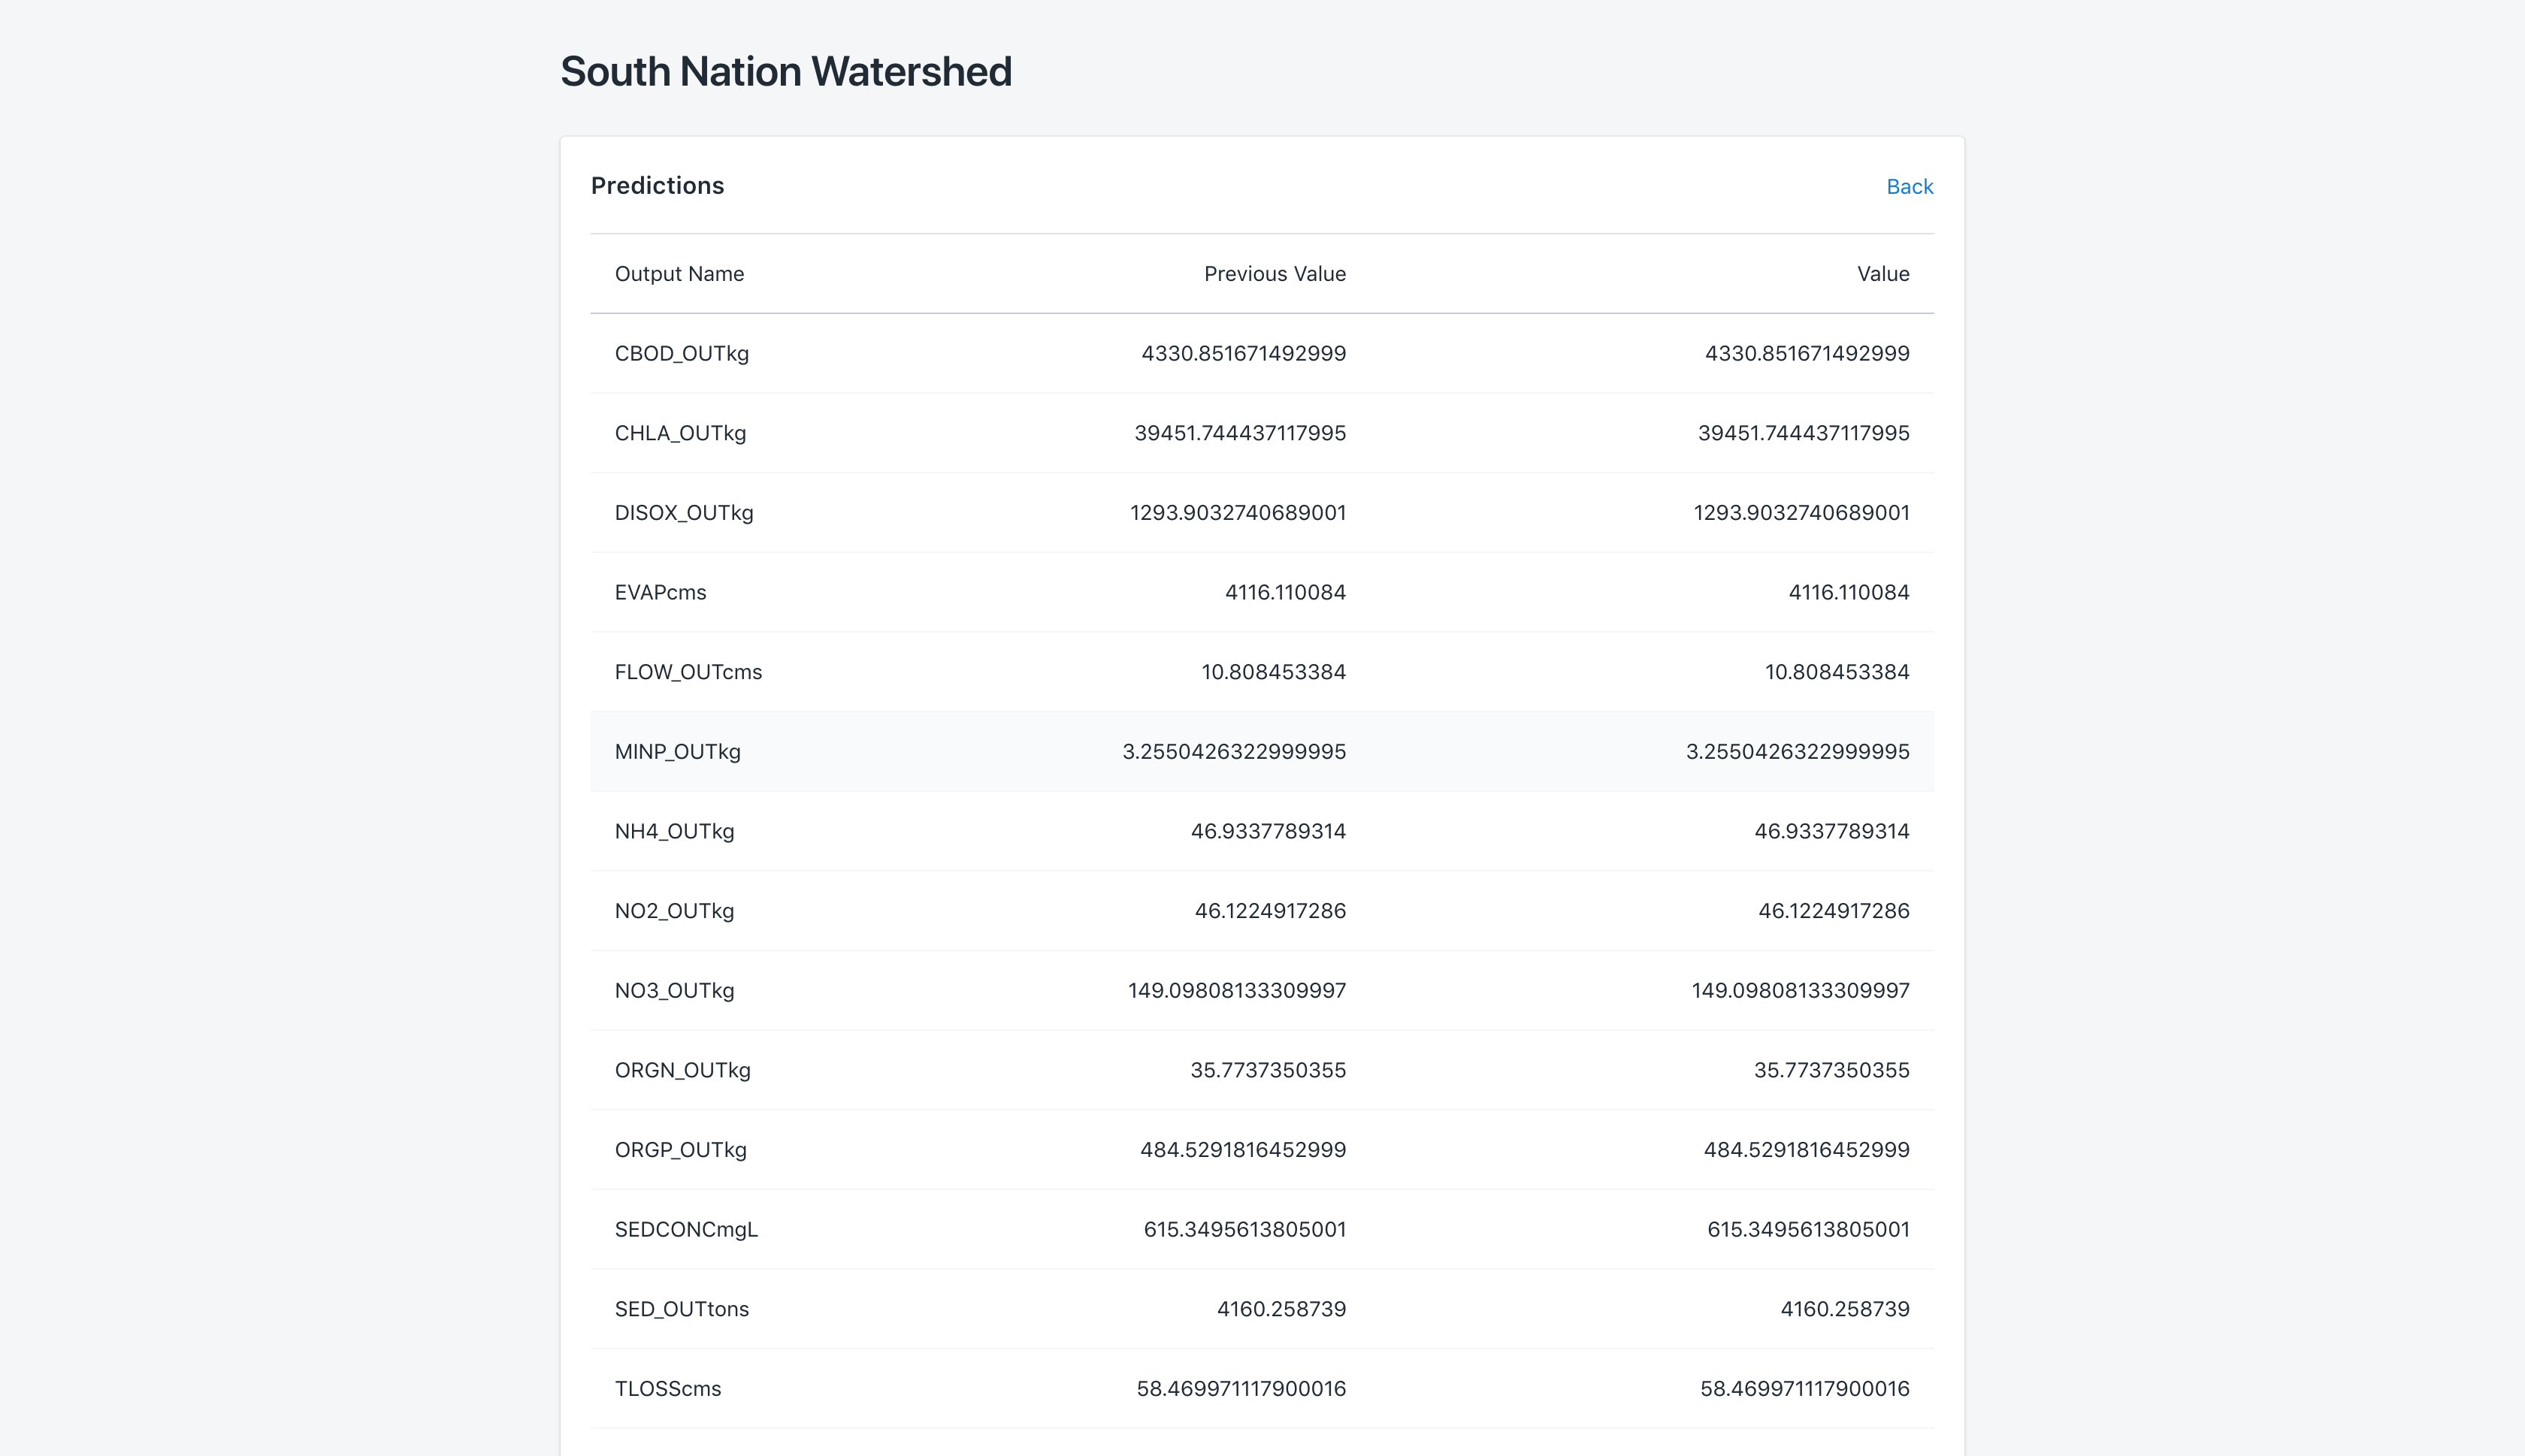
\includegraphics[width=\linewidth]{images/webpage.png}
\endminipage
\caption{The predicted changes in downstream runoff metrics based on precipitation and forest cover inputs, as presented to the user.} \label{fig-web}
\end{center}
\end{figure}

\subsection{Projected Changes in Hydrological Variables}
% Graphs
The random forest models were used to predict changes in downstream runoff values given a range of - 50\% to + 50\%change in forest cover or a range of -15\% to + 15\% change in precipitation across the watershed, which are within the range of observed values.
Random forest regression models are inherently poor at extrapolating outside of data seen in its training set due to the branching and averaging of nodes, and the generated predictor values were chosen to be within this range.
The individual predictions as a factor of percent change from baseline are provided in Figure \ref{fig-fc} for changes in forest cover and Figure \ref{fig-pcp} for changes in precipitation.

\begin{figure}[h]
\begin{center}
\minipage{0.7\textwidth}%
  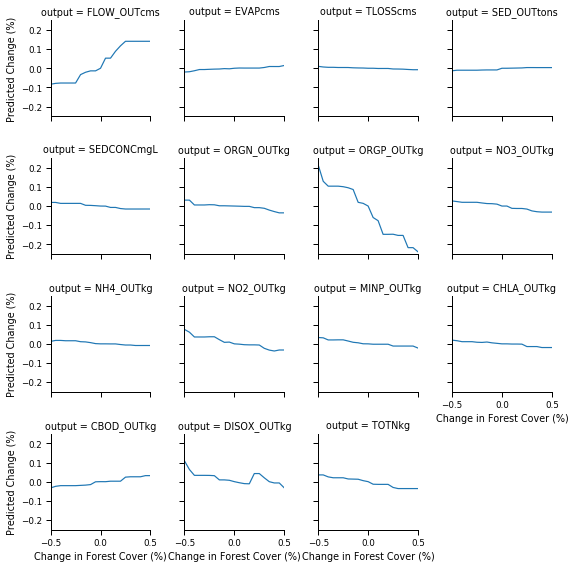
\includegraphics[width=\linewidth]{images/predictions_forest_facetgrid.png}
\endminipage
\caption{Predicted percent changes given a -50\% to +50\% change in the watershed's overall forest cover.} \label{fig-fc}
\end{center}
\end{figure}

\begin{figure}[h]
\begin{center}
\minipage{0.7\textwidth}%
  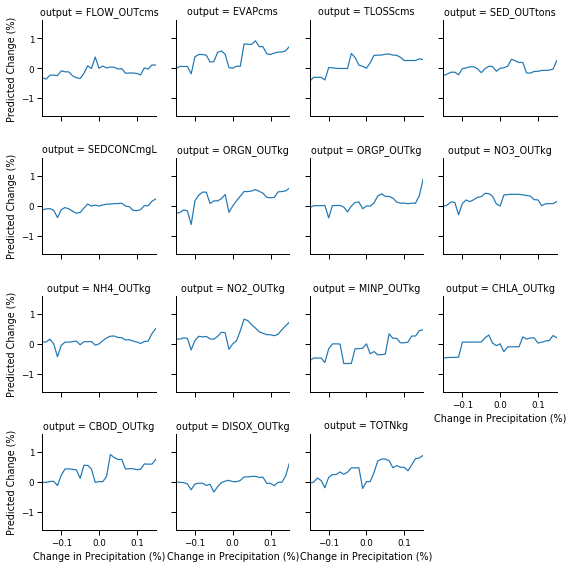
\includegraphics[width=\linewidth]{images/predictions_precipitation_facetgrid.png}
\endminipage
\caption{Predicted percent changes given a -15\% to +15\% change in the watershed's overall forest cover.} \label{fig-pcp}
\end{center}
\end{figure}

\subsection{Model Accuracy}
Table \ref{rf_accuracies} provides a summary of the models' accuracies in predicting various downstream measures.
The accuracies were determined using a Time Series Split where the temporal ordering is kept between training and test data sets.
For example, with a dataset consisting of years 2000 to 2005 inclusive, a time series split might create a training set with year 2000, 2001, 2002 and test set with year 2003.
As shown, the random forest models performed poorly for predicting water outflow rate (FLOW\_OUTcms) and organic phosphorous outflow (ORGP\_OUTkg).
That is, if the models were trained with x sets of prior years, the models are poor at predicting a future year's water outflow or organic phosphorous outflow.
The model performed significantly better for predicting the other measures: evaporation rate, water transmission loss rate, sediment output, sediment concentration, organic nitrogen output, nitrate output, ammonium output, nitrogen dioxide output, mineral phosphorus output, chlorophyll alpha output, carbonaceous biochemical oxygen demand of material output, dissolved oxygen output, and total nitrogen in surface runoff.

% Table
\small \begin{table}[h]
\caption{Accuracy of random forest models for the downstream predictands.}
\label{rf_accuracies}
\centering
% \resizebox{\textwidth}{!}{%
\begin{tabular}{lll}
 & accuracy & standard deviation \\
FLOW\_OUTcms & 0.77453974177041 & 0.2294149291032354 \\
EVAPcms & 0.9697462141575514 & 0.03342663731811072 \\
TLOSScms & 0.9849085443489066 & 0.015783200164635483 \\
SED\_OUTtons & 0.9669386142355473 & 0.031369149259199765 \\
SEDCONCmgL & 0.9550856665204039 & 0.04719784299228629 \\
ORGN\_OUTkg & 0.9485722009887052 & 0.0513537106801331 \\
ORGP\_OUTkg & 0.8288877495883687 & 0.21551718529974206 \\
NO3\_OUTkg & 0.960748053541662 & 0.03156239767529165 \\
NH4\_OUTkg & 0.9505648610245114 & 0.04504648732478451 \\
NO2\_OUTkg & 0.9166867771433014 & 0.08570031297945056 \\
MINP\_OUTkg & 0.9692740147487756 & 0.027323554055449954 \\
CHLA\_OUTkg & 0.9709013616816519 & 0.02554074062863536 \\
CBOD\_OUTkg & 0.9707570596314152 & 0.02727914422698616 \\
DISOX\_OUTkg & 0.9234165773438077 & 0.07587513874148259 \\
TOTNkg & 0.9172299325385997 & 0.09975026057106322
\end{tabular}%
% }
\end{table}


\section{Conclusions}

% For citations of references, we prefer the use of square brackets
% and consecutive numbers. Citations using labels or the author/year
% convention are also acceptable. The following bibliography provides
% a sample reference list with entries for journal
% articles~\cite{ref_article1}, an LNCS chapter~\cite{ref_lncs1}, a
% book~\cite{ref_book1}, proceedings without editors~\cite{ref_proc1},
% and a homepage~\cite{ref_url1}. Multiple citations are grouped
% \cite{ref_article1,ref_lncs1,ref_book1},
% \cite{ref_article1,ref_book1,ref_proc1,ref_url1}.
%
% ---- Bibliography ----
%
% BibTeX users should specify bibliography style 'splncs04'.c v
% References will then be sorted and formatted in the correct style.
%
% \bibliographystyle{splncs04}
% \bibliography{mybibliography}
%
\begin{thebibliography}{8}
% \bibitem{ref_article1}
% Author, F.: Article title. Journal \textbf{2}(5), 99--110 (2016)

% \bibitem{ref_lncs1}
% Author, F., Author, S.: Title of a proceedings paper. In: Editor,
% F., Editor, S. (eds.) CONFERENCE 2016, LNCS, vol. 9999, pp. 1--13.
% Springer, Heidelberg (2016). \doi{10.10007/1234567890}

% \bibitem{ref_book1}
% Author, F., Author, S., Author, T.: Book title. 2nd edn. Publisher,
% Location (1999)

% \bibitem{ref_proc1}
% Author, A.-B.: Contribution title. In: 9th International Proceedings
% on Proceedings, pp. 1--2. Publisher, Location (2010)

% \bibitem{ref_url1}
% LNCS Homepage, \url{http://www.springer.com/lncs}. Last accessed 4
% Oct 2017
\end{thebibliography}
\end{document}
